% Kommentare für den Editor (TexWorks/TexMakerX)
% !TeX encoding   = utf8
% !TeX spellcheck = de-DE

% --- LaTeX Vorlage ------------------------------------------------------
% speziell für einfache Dokumente wie Praktikumsprotokolle
%
% Autor: Matthias Pospiech (matthias@pospiech.eu)
% ------------------------------------------------------------------------

% Dokumentenklasse (Koma Script) -----------------------------------------
\documentclass[%
   %draft,     % Entwurfsstadium
   final,      % fertiges Dokument
   paper=a4, paper=portrait, pagesize=auto, % Papier Einstellungen
   fontsize=11pt, % Schriftgröße
   ngerman, % Sprache 
 ]{scrreprt} % Classes: scrartcl, scrreprt, scrbook

% ~~~~~~~~~~~~~~~~~~~~~~~~~~~~~~~~~~~~~~~~~~~~~~~~~~~~~~~~~~~~~~~~~~~~~~~~
% encoding
% ~~~~~~~~~~~~~~~~~~~~~~~~~~~~~~~~~~~~~~~~~~~~~~~~~~~~~~~~~~~~~~~~~~~~~~~~

% Encoding der Dateien (sonst funktionieren Umlaute nicht)
\usepackage[utf8]{inputenc}

% Encoding der Verzeichnisse (für Pfade mit Umlauten und Leerzeichne)
\usepackage[%
   extendedchars, encoding, multidot, space,
   %filenameencoding=latin1, % Windows XP, Vista, 7
   filenameencoding=utf8,   % Linux, OS X
]{grffile}

% ~~~~~~~~~~~~~~~~~~~~~~~~~~~~~~~~~~~~~~~~~~~~~~~~~~~~~~~~~~~~~~~~~~~~~~~~
% Pakete und Stile
% ~~~~~~~~~~~~~~~~~~~~~~~~~~~~~~~~~~~~~~~~~~~~~~~~~~~~~~~~~~~~~~~~~~~~~~~~
% Schriften
% ~~~~~~~~~~~~~~~~~~~~~~~~~~~~~~~~~~~~~~~~~~~~~~~~~~~~~~~~~~~~~~~~~~~~~~~~
% Fonts Fonts Fonts
% ~~~~~~~~~~~~~~~~~~~~~~~~~~~~~~~~~~~~~~~~~~~~~~~~~~~~~~~~~~~~~~~~~~~~~~~~

% immer laden:
\usepackage[T1]{fontenc} % T1 Schrift Encoding
\usepackage{textcomp}	 % Zusätzliche Symbole (Text Companion font extension)

% ~~~~~~~~~~~~~~~~~~~~~~~~~~~~~~~~~~~~~~~~~~~~~~~~~~~~~~~~~~~~~~~~~~~~~~~~
% Symbole
% ~~~~~~~~~~~~~~~~~~~~~~~~~~~~~~~~~~~~~~~~~~~~~~~~~~~~~~~~~~~~~~~~~~~~~~~~

\usepackage{amssymb}
\usepackage{mathcomp}


%% ==== Zusammengesetzte Schriften  (Sans + Serif) =======================

%% - Latin Modern
\usepackage{lmodern}
%% -------------------

%% - Bera Schriften
%\usepackage{bera}
%% -------------------

%% - Times, Helvetica, Courier (Word Standard...)
%\usepackage{mathptmx}
%\usepackage[scaled=.90]{helvet}
%\usepackage{courier}
%% -------------------

%% - Palantino , Helvetica, Courier
%\usepackage{mathpazo}
%\usepackage[scaled=.95]{helvet}
%\usepackage{courier}
%% -------------------

%% - Charter, Bera Sans
%\usepackage{charter}\linespread{1.05}
%\renewcommand{\sfdefault}{fvs}
%\usepackage[charter]{mathdesign}



%%%% =========== Typewriter =============

%\usepackage{courier}                   %% --- Courier
%\renewcommand{\ttdefault}{cmtl}        %% --- CmBright Typewriter Font
%\usepackage[%                          %% --- Luxi Mono (Typewriter)
%   scaled=0.9
%]{luximono}



% Pakete Laden
% ~~~~~~~~~~~~~~~~~~~~~~~~~~~~~~~~~~~~~~~~~~~~~~~~~~~~~~~~~~~~~~~~~~~~~~~~
% These packages must be loaded before all others
% (primarily because they are required by other packages)
% ~~~~~~~~~~~~~~~~~~~~~~~~~~~~~~~~~~~~~~~~~~~~~~~~~~~~~~~~~~~~~~~~~~~~~~~~
\usepackage{calc}
\usepackage{fixltx2e}	% Fix known LaTeX2e bugs

\usepackage[ngerman]{babel} 	% Sprache
\usepackage[dvipsnames, table]{xcolor} 	% Farben
\usepackage[ngerman, iso]{isodate} 	%Datumsformat

% ~~~~~~~~~~~~~~~~~~~~~~~~~~~~~~~~~~~~~~~~~~~~~~~~~~~~~~~~~~~~~~~~~~~~~~~~
% Bilder, Gleitumgebungen und Platzierung
% ~~~~~~~~~~~~~~~~~~~~~~~~~~~~~~~~~~~~~~~~~~~~~~~~~~~~~~~~~~~~~~~~~~~~~~~~

\usepackage[]{graphicx}					% Graphiken
\usepackage{epstopdf}		% konvertiert eps in pdf

% provides new floats and enables H float modifier option
\usepackage{float}
% Floats immer erst nach der Referenz setzen
\usepackage{flafter}
% Alel Floats werden vor der nächsten section ausgegeben
\usepackage[section]{placeins} 
%

\usepackage{tikz}
%tikz verwenden um Grafiken zu erstellen
\usepackage{pgfplots}
%pgfplots verwenden für Diagramme

\usepackage[european, siunitx]{circuitikz}
% Schaltpläne

% ~~~~~~~~~~~~~~~~~~~~~~~~~~~~~~~~~~~~~~~~~~~~~~~~~~~~~~~~~~~~~~~~~~~~~~~~
% Beschriftungen (captions)
% ~~~~~~~~~~~~~~~~~~~~~~~~~~~~~~~~~~~~~~~~~~~~~~~~~~~~~~~~~~~~~~~~~~~~~~~~

\usepackage{caption}
\usepackage{subcaption}

% ~~~~~~~~~~~~~~~~~~~~~~~~~~~~~~~~~~~~~~~~~~~~~~~~~~~~~~~~~~~~~~~~~~~~~~~~
% Math
% ~~~~~~~~~~~~~~~~~~~~~~~~~~~~~~~~~~~~~~~~~~~~~~~~~~~~~~~~~~~~~~~~~~~~~~~~

% Base Math Package
\usepackage[fleqn]{amsmath} 
% Warnt bei Benutzung von Befehlen die mit amsmath inkompatibel sind.
\usepackage[all, error]{onlyamsmath}
%Brüche schräg statt horizontal brechen
\usepackage{nicefrac}

% ~~~~~~~~~~~~~~~~~~~~~~~~~~~~~~~~~~~~~~~~~~~~~~~~~~~~~~~~~~~~~~~~~~~~~~~~
% Science
% ~~~~~~~~~~~~~~~~~~~~~~~~~~~~~~~~~~~~~~~~~~~~~~~~~~~~~~~~~~~~~~~~~~~~~~~~

% Einheiten und Zahlenformatierung
\usepackage{siunitx}

% ~~~~~~~~~~~~~~~~~~~~~~~~~~~~~~~~~~~~~~~~~~~~~~~~~~~~~~~~~~~~~~~~~~~~~~~~
% Tables (Tabular)
% ~~~~~~~~~~~~~~~~~~~~~~~~~~~~~~~~~~~~~~~~~~~~~~~~~~~~~~~~~~~~~~~~~~~~~~~~

\usepackage{booktabs}
\usepackage{ltxtable} % Longtable + tabularx

% ~~~~~~~~~~~~~~~~~~~~~~~~~~~~~~~~~~~~~~~~~~~~~~~~~~~~~~~~~~~~~~~~~~~~~~~~
% text related packages
% ~~~~~~~~~~~~~~~~~~~~~~~~~~~~~~~~~~~~~~~~~~~~~~~~~~~~~~~~~~~~~~~~~~~~~~~~

\usepackage{url}            % Befehl \url{...}
\usepackage{enumitem}		% Kompakte Listen

% Neue Befehle: \Centering, \RaggedLeft, and \RaggedRight, ... 
\usepackage{ragged2e}


% ~~~~~~~~~~~~~~~~~~~~~~~~~~~~~~~~~~~~~~~~~~~~~~~~~~~~~~~~~~~~~~~~~~~~~~~~
% Citations
% ~~~~~~~~~~~~~~~~~~~~~~~~~~~~~~~~~~~~~~~~~~~~~~~~~~~~~~~~~~~~~~~~~~~~~~~~

%\usepackage[
%	style=alphabetic, % Loads the bibliography and the citation style 
%	natbib=true, % define natbib compatible cite commands
%]{biblatex}	
% Other options:
%	style=numeric, % 
%	style=numeric-comp,    % [1–3, 7, 8]
%	style=numeric-verb,    % [2]; [5]; [6]

\usepackage{csquotes}

% ~~~~~~~~~~~~~~~~~~~~~~~~~~~~~~~~~~~~~~~~~~~~~~~~~~~~~~~~~~~~~~~~~~~~~~~~
% layout packages
% ~~~~~~~~~~~~~~~~~~~~~~~~~~~~~~~~~~~~~~~~~~~~~~~~~~~~~~~~~~~~~~~~~~~~~~~~
%
% Befehle für 1,5 und 2 zeilig: 
% \singlespacing, \onehalfspacing und \doublespacing
\usepackage{setspace}

% ~~~~~~~~~~~~~~~~~~~~~~~~~~~~~~~~~~~~~~~~~~~~~~~~~~~~~~~~~~~~~~~~~~~~~~~~
% Kopf und Fusszeile
% ~~~~~~~~~~~~~~~~~~~~~~~~~~~~~~~~~~~~~~~~~~~~~~~~~~~~~~~~~~~~~~~~~~~~~~~~

% Kopf und Fusszeile mit scrpage2 einstellen
\usepackage[automark, komastyle, nouppercase]{scrpage2}

% ~~~~~~~~~~~~~~~~~~~~~~~~~~~~~~~~~~~~~~~~~~~~~~~~~~~~~~~~~~~~~~~~~~~~~~~~
% pdf packages
% ~~~~~~~~~~~~~~~~~~~~~~~~~~~~~~~~~~~~~~~~~~~~~~~~~~~~~~~~~~~~~~~~~~~~~~~~

% Include pages from external PDF documents in LaTeX documents
\usepackage{pdfpages} 

% Optischer Randausgleich mit pdfTeX
\usepackage{microtype}

%%% svg to tex
\newcommand{\executeiffilenewer}[3]{%
\ifnum\pdfstrcmp{\pdffilemoddate{#1}}%
{\pdffilemoddate{#2}}>0%
{\immediate\write18{#3}}\fi%
}

% Einstellungen und Layoutstile 
% ~~~~~~~~~~~~~~~~~~~~~~~~~~~~~~~~~~~~~~~~~~~~~~~~~~~~~~~~~~~~~~~~~~~~~~~~
% Colors
% ~~~~~~~~~~~~~~~~~~~~~~~~~~~~~~~~~~~~~~~~~~~~~~~~~~~~~~~~~~~~~~~~~~~~~~~~
\definecolor{sectioncolor}{RGB}{0, 0, 0}     % black

% ~~~~~~~~~~~~~~~~~~~~~~~~~~~~~~~~~~~~~~~~~~~~~~~~~~~~~~~~~~~~~~~~~~~~~~~~
% text related 
% ~~~~~~~~~~~~~~~~~~~~~~~~~~~~~~~~~~~~~~~~~~~~~~~~~~~~~~~~~~~~~~~~~~~~~~~~

%% style of URL
\urlstyle{tt}


% Keine hochgestellten Ziffern in der Fussnote (KOMA-Script-spezifisch):
\deffootnote{1.5em}{1em}{\makebox[1.5em][l]{\thefootnotemark}}

% Limit space of footnotes to 10 lines
\setlength{\dimen\footins}{10\baselineskip}

% prevent continuation of footnotes 
% at facing page
\interfootnotelinepenalty=10000 

% ~~~~~~~~~~~~~~~~~~~~~~~~~~~~~~~~~~~~~~~~~~~~~~~~~~~~~~~~~~~~~~~~~~~~~~~~
% Science
% ~~~~~~~~~~~~~~~~~~~~~~~~~~~~~~~~~~~~~~~~~~~~~~~~~~~~~~~~~~~~~~~~~~~~~~~~

\sisetup{%
	mode = math, detect-family, detect-weight,	
	exponent-product = \cdot,
	number-unit-separator=\text{\,},
	output-decimal-marker={,},
}

% ~~~~~~~~~~~~~~~~~~~~~~~~~~~~~~~~~~~~~~~~~~~~~~~~~~~~~~~~~~~~~~~~~~~~~~~~
% Citations / Style of Bibliography
% ~~~~~~~~~~~~~~~~~~~~~~~~~~~~~~~~~~~~~~~~~~~~~~~~~~~~~~~~~~~~~~~~~~~~~~~~

% Kommentar entfernene wenn biblatex geladen wird
% \IfPackageLoaded{biblatex}{%
	\ExecuteBibliographyOptions{%
%--- Backend --- --- ---
	backend=bibtex,  % (bibtex, bibtex8, biber)
	bibwarn=true, %
	bibencoding=ascii, % (ascii, inputenc, <encoding>)
%--- Sorting --- --- ---
	sorting=nty, % Sort by name, title, year.
	% other options: 
	% nty        Sort by name, title, year.
	% nyt        Sort by name, year, title.
	% nyvt       Sort by name, year, volume, title.
	% anyt       Sort by alphabetic label, name, year, title.
	% anyvt      Sort by alphabetic label, name, year, volume, title.
	% ynt        Sort by year, name, title.
	% ydnt       Sort by year (descending), name, title.
	% none       Do not sort at all. All entries are processed in citation order.
	% debug      Sort by entry key. This is intended for debugging only.
	%
	sortcase=true,
	sortlos=los, % (bib, los) The sorting order of the list of shorthands
	sortcites=false, % do/do not sort citations according to bib	
%--- Dates --- --- ---
	date=comp,  % (short, long, terse, comp, iso8601)
%	origdate=
%	eventdate=
%	urldate=
%	alldates=
	datezeros=true, %
	dateabbrev=true, %
%--- General Options --- --- ---
	maxnames=1,
	minnames=1,
%	maxbibnames=99,
%	maxcitenames=1,
%	autocite= % (plain, inline, footnote, superscript) 
	autopunct=true,
	language=auto,
	babel=none, % (none, hyphen, other, other*)
	block=none, % (none, space, par, nbpar, ragged)
	notetype=foot+end, % (foot+end, footonly, endonly)
	hyperref=true, % (true, false, auto)
	backref=true,
	backrefstyle=three, % (none, three, two, two+, three+, all+)
	backrefsetstyle=setonly, %
	indexing=false, % 
	% options:
	% true       Enable indexing globally.
	% false      Disable indexing globally.
	% cite       Enable indexing in citations only.
	% bib        Enable indexing in the bibliography only.
	refsection=none, % (part, chapter, section, subsection)
	refsegment=none, % (none, part, chapter, section, subsection)
	abbreviate=true, % (true, false)
	defernumbers=false, % 
	punctfont=false, % 
	arxiv=abs, % (ps, pdf, format)	
%--- Style Options --- --- ---	
% The following options are provided by the standard styles
	isbn=false,%
	url=false,%
	doi=false,%
	eprint=false,%	
	}%	
	
	% change alpha label to be without +	
	\renewcommand*{\labelalphaothers}{}
	
	% change 'In: <magazine>" to "<magazine>"
	\renewcommand*{\intitlepunct}{}
	\DefineBibliographyStrings{german}{in={}}
	
	% make names capitalized \textsc{}
	\renewcommand{\mkbibnamefirst}{\textsc}
	\renewcommand{\mkbibnamelast}{\textsc}
	
	% make volume and number look like 
	% 'Bd. 33(14): '
	\renewbibmacro*{volume+number+eid}{%
	  \setunit{\addcomma\space}%
	  \bibstring{volume}% 
	  \setunit{\addspace}%
	  \printfield{volume}%
	  \iffieldundef{number}{}{% 
	    \printtext[parens]{%
	      \printfield{number}%
	    }%
	  }%
	  \setunit{\addcomma\space}%
	  \printfield{eid}
	  %\setunit{\addcolon\space}%
	  }	

	% <authors>: <title>
	\renewcommand*{\labelnamepunct}{\addcolon\space}
	% make ': ' before pages
	\renewcommand*{\bibpagespunct}{\addcolon\space}
	% names delimiter ';' instead of ','
	%\renewcommand*{\multinamedelim}{\addsemicolon\space}

	% move date before issue
	\renewbibmacro*{journal+issuetitle}{%
	  \usebibmacro{journal}%
	  \setunit*{\addspace}%
	  \iffieldundef{series}
	    {}
	    {\newunit
	     \printfield{series}%
	     \setunit{\addspace}}%
	  %
	  \usebibmacro{issue+date}%
	  \setunit{\addcolon\space}%
	  \usebibmacro{issue}%
	  \setunit{\addspace}%
	  \usebibmacro{volume+number+eid}%
	  \newunit}

	% print all names, even if maxnames = 1
	\DeclareCiteCommand{\citeauthors}
	  {
	   \defcounter{maxnames}{1000}
	   \boolfalse{citetracker}%
	   \boolfalse{pagetracker}%
	   \usebibmacro{prenote}}
	  {\ifciteindex
	     {\indexnames{labelname}}
	     {}%
	   \printnames{labelname}}
	  {\multicitedelim}
	  {\usebibmacro{postnote}}

}%

% ~~~~~~~~~~~~~~~~~~~~~~~~~~~~~~~~~~~~~~~~~~~~~~~~~~~~~~~~~~~~~~~~~~~~~~~~
% figures, placement, floats and captions
% ~~~~~~~~~~~~~~~~~~~~~~~~~~~~~~~~~~~~~~~~~~~~~~~~~~~~~~~~~~~~~~~~~~~~~~~~

% Make float placement easier
\renewcommand{\floatpagefraction}{.75} % vorher: .5
\renewcommand{\textfraction}{.1}       % vorher: .2
\renewcommand{\topfraction}{.8}        % vorher: .7
\renewcommand{\bottomfraction}{.5}     % vorher: .3
\setcounter{topnumber}{3}        % vorher: 2
\setcounter{bottomnumber}{2}     % vorher: 1
\setcounter{totalnumber}{5}      % vorher: 3

%% ~~~ Captions ~~~~~~~~~~~~~~~~~~~~~~~~~~~~~~~~~~~~~~~~~~~~~~~~~~~~~~~~~~
% Style of captions
\DeclareCaptionStyle{captionStyleTemplateDefault}
[ % single line captions
   justification = centering
]
{ % multiline captions
% -- Formatting
   format      = plain,  % plain, hang
   indention   = 0em,    % indention of text 
   labelformat = default,% default, empty, simple, brace, parens
   labelsep    = colon,  % none, colon, period, space, quad, newline, endash
   textformat  = simple, % simple, period
% -- Justification
   justification = justified, %RaggedRight, justified, centering
   singlelinecheck = true, % false (true=ignore justification setting in single line)
% -- Fonts
   labelfont   = {small,bf},
   textfont    = {small,rm},
% valid values:
% scriptsize, footnotesize, small, normalsize, large, Large
% normalfont, ip, it, sl, sc, md, bf, rm, sf, tt
% singlespacing, onehalfspacing, doublespacing
% normalcolor, color=<...>
%
% -- Margins and further paragraph options
   margin = 10pt, %.1\textwidth,
   % width=.8\linewidth,
% -- Skips
   skip     = 10pt, % vertical space between the caption and the figure
   position = auto, % top, auto, bottom
% -- Lists
   % list=no, % suppress any entry to list of figure 
   listformat = subsimple, % empty, simple, parens, subsimple, subparens
% -- Names & Numbering
   % figurename = Abb. %
   % tablename  = Tab. %
   % listfigurename=
   % listtablename=
   % figurewithin=chapter
   % tablewithin=chapter
%-- hyperref related options
	hypcap=true, % (true, false) 
	% true=all hyperlink anchors are placed at the 
	% beginning of the (floating) environment
	%
	hypcapspace=0.5\baselineskip
}

% apply caption style
\captionsetup{
	style = captionStyleTemplateDefault % base
}

% Predefinded skip setup for different floats
\captionsetup[table]{position=top}
\captionsetup[figure]{position=bottom}


% options for subcaptions
\captionsetup[sub]{ %
	style = captionStyleTemplateDefault, % base
	skip=6pt,
	margin=5pt,
	labelformat = parens,% default, empty, simple, brace
	labelsep    = space,
	list=false,
	hypcap=false
}

% ~~~~~~~~~~~~~~~~~~~~~~~~~~~~~~~~~~~~~~~~~~~~~~~~~~~~~~~~~~~~~~~~~~~~~~~~
% layout 
% ~~~~~~~~~~~~~~~~~~~~~~~~~~~~~~~~~~~~~~~~~~~~~~~~~~~~~~~~~~~~~~~~~~~~~~~~


%% Paragraph Separation =================================
\KOMAoptions{%
   parskip=absolute, % do not change indentation according to fontsize
   parskip=false     % indentation of 1em
   % parskip=half    % parksip of 1/2 line 
}%

%% line spacing =========================================
%\onehalfspacing	% 1,5-facher Abstand
%\doublespacing		% 2-facher Abstand

%% page layout ==========================================

\raggedbottom     % Variable Seitenhoehen zulassen

% Koma Script text area layout
\KOMAoptions{%
   DIV=11,% (Size of Text Body, higher values = greater textbody)
   BCOR=5mm% (Bindekorrektur)
}%

%%% === Page Layout  Options ===
\KOMAoptions{% (most options are for package typearea)
   % twoside=true, % two side layout (alternating margins, standard in books)
   twoside=false, % single side layout 
   %
   headlines=2.1,%
}%

%\KOMAoptions{%
%      headings=noappendixprefix % chapter in appendix as in body text
%      ,headings=nochapterprefix  % no prefix at chapters
%      % ,headings=appendixprefix   % inverse of 'noappendixprefix'
%      % ,headings=chapterprefix    % inverse of 'nochapterprefix'
%      % ,headings=openany   % Chapters start at any side
%      % ,headings=openleft  % Chapters start at left side
%      ,headings=openright % Chapters start at right side      
%}%


% reloading of typearea, necessary if setting of spacing changed
\typearea[current]{last}

%% Zitate
\renewcommand*{\dictumwidth}{0.5\textwidth}

% ~~~~~~~~~~~~~~~~~~~~~~~~~~~~~~~~~~~~~~~~~~~~~~~~~~~~~~~~~~~~~~~~~~~~~~~~
% Titlepage
% ~~~~~~~~~~~~~~~~~~~~~~~~~~~~~~~~~~~~~~~~~~~~~~~~~~~~~~~~~~~~~~~~~~~~~~~~
\KOMAoptions{%
   % titlepage=true %
   titlepage=false %
}%

% ~~~~~~~~~~~~~~~~~~~~~~~~~~~~~~~~~~~~~~~~~~~~~~~~~~~~~~~~~~~~~~~~~~~~~~~~
% head and foot lines
% ~~~~~~~~~~~~~~~~~~~~~~~~~~~~~~~~~~~~~~~~~~~~~~~~~~~~~~~~~~~~~~~~~~~~~~~~

% \pagestyle{scrheadings} % Seite mit Headern
\pagestyle{scrplain} % Seiten ohne Header

% loescht voreingestellte Stile
\clearscrheadings
\clearscrplain
%
% Was steht wo...
% Bei headings:
%   % Oben aussen: Kapitel und Section
%   % Unten aussen: Seitenzahl
%   \ohead{\pagemark}
%   \ihead{\headmark}
%   \ofoot[\pagemark]{} % Außen unten: Seitenzahlen bei plain
% Bei Plain:
\cfoot[\pagemark]{\pagemark} % Mitte unten: Seitenzahlen bei plain


% Angezeigte Abschnitte im Header
% \automark[section]{chapter} %[rechts]{links}
\automark[subsection]{section} %[rechts]{links}

% ~~~~~~~~~~~~~~~~~~~~~~~~~~~~~~~~~~~~~~~~~~~~~~~~~~~~~~~~~~~~~~~~~~~~~~~~
% headings / page opening
% ~~~~~~~~~~~~~~~~~~~~~~~~~~~~~~~~~~~~~~~~~~~~~~~~~~~~~~~~~~~~~~~~~~~~~~~~
\setcounter{secnumdepth}{3}

\KOMAoptions{%
%%%% headings
   % headings=small  % Small Font Size, thin spacing above and below
   % headings=normal % Medium Font Size, medium spacing above and below
   headings=big % Big Font Size, large spacing above and below
}%

% Titelzeile linksbuendig, haengend
\renewcommand*{\raggedsection}{\raggedright} 

% ~~~~~~~~~~~~~~~~~~~~~~~~~~~~~~~~~~~~~~~~~~~~~~~~~~~~~~~~~~~~~~~~~~~~~~~~
% fonts of headings
% ~~~~~~~~~~~~~~~~~~~~~~~~~~~~~~~~~~~~~~~~~~~~~~~~~~~~~~~~~~~~~~~~~~~~~~~~
\setkomafont{sectioning}{\normalfont\sffamily} % \rmfamily
\setkomafont{descriptionlabel}{\itshape}
\setkomafont{pageheadfoot}{\normalfont\normalcolor\small\sffamily}
\setkomafont{pagenumber}{\normalfont\sffamily}

%%% --- Titlepage ---
%\setkomafont{subject}{}
%\setkomafont{subtitle}{}
%\setkomafont{title}{}

% ~~~~~~~~~~~~~~~~~~~~~~~~~~~~~~~~~~~~~~~~~~~~~~~~~~~~~~~~~~~~~~~~~~~~~~~~
% settings and layout of TOC, LOF, 
% ~~~~~~~~~~~~~~~~~~~~~~~~~~~~~~~~~~~~~~~~~~~~~~~~~~~~~~~~~~~~~~~~~~~~~~~~
\setcounter{tocdepth}{3} % Depth of TOC Display

% ~~~~~~~~~~~~~~~~~~~~~~~~~~~~~~~~~~~~~~~~~~~~~~~~~~~~~~~~~~~~~~~~~~~~~~~~
% Tabellen
% ~~~~~~~~~~~~~~~~~~~~~~~~~~~~~~~~~~~~~~~~~~~~~~~~~~~~~~~~~~~~~~~~~~~~~~~~

%%% -| Neue Spaltendefinitionen 'columntypes' |--
%
% Belegte Spaltentypen:
% l - links
% c - zentriert
% r - rechts
% p,m,b  - oben, mittig, unten
% X - tabularx Auto-Spalte

% um Tabellenspalten mit Flattersatz zu setzen, muss \\ vor
% (z.B.) \raggedright geschuetzt werden:
\newcommand{\PreserveBackslash}[1]{\let\temp=\\#1\let\\=\temp}

% Spalten mit Flattersatz und definierte Breite:
% m{} -> mittig
% p{} -> oben
% b{} -> unten
%
% Linksbuendig:
\newcolumntype{v}[1]{>{\PreserveBackslash\RaggedRight\hspace{0pt}}p{#1}}
\newcolumntype{M}[1]{>{\PreserveBackslash\RaggedRight\hspace{0pt}}m{#1}}
% % Rechtsbuendig :
% \newcolumntype{R}[1]{>{\PreserveBackslash\RaggedLeft\hspace{0pt}}m{#1}}
% \newcolumntype{S}[1]{>{\PreserveBackslash\RaggedLeft\hspace{0pt}}p{#1}}
% % Zentriert :
% \newcolumntype{Z}[1]{>{\PreserveBackslash\Centering\hspace{0pt}}m{#1}}
% \newcolumntype{A}[1]{>{\PreserveBackslash\Centering\hspace{0pt}}p{#1}}

\newcolumntype{Y}{>{\PreserveBackslash\RaggedLeft\hspace{0pt}}X}

%-- Einstellungen für Tabellen ----------
\providecommand\tablestyle{%
  \renewcommand{\arraystretch}{1.4} % Groessere Abstaende zwischen Zeilen
  \normalfont\normalsize            %
  \sffamily\small           % Serifenlose und kleine Schrift
  \centering%                       % Tabelle zentrieren
}

%--Einstellungen für Tabellen ----------

\colorlet{tablesubheadcolor}{gray!40}
\colorlet{tableheadcolor}{gray!25}
\colorlet{tableblackheadcolor}{black!60}
\colorlet{tablerowcolor}{gray!15.0}


% ~~~~~~~~~~~~~~~~~~~~~~~~~~~~~~~~~~~~~~~~~~~~~~~~~~~~~~~~~~~~~~~~~~~~~~~~
% pdf packages
% ~~~~~~~~~~~~~~~~~~~~~~~~~~~~~~~~~~~~~~~~~~~~~~~~~~~~~~~~~~~~~~~~~~~~~~~~

% ~~~~~~~~~~~~~~~~~~~~~~~~~~~~~~~~~~~~~~~~~~~~~~~~~~~~~~~~~~~~~~~~~~~~~~~~
% fix remaining problems
% ~~~~~~~~~~~~~~~~~~~~~~~~~~~~~~~~~~~~~~~~~~~~~~~~~~~~~~~~~~~~~~~~~~~~~~~~




% ~~~~~~~~~~~~~~~~~~~~~~~~~~~~~~~~~~~~~~~~~~~~~~~~~~~~~~~~~~~~~~~~~~~~~~~~
% Eigene Befehle
% ~~~~~~~~~~~~~~~~~~~~~~~~~~~~~~~~~~~~~~~~~~~~~~~~~~~~~~~~~~~~~~~~~~~~~~~~
% -- new commands --
\providecommand{\abs}[1]{\lvert#1\rvert}
\providecommand{\Abs}[1]{\left\lvert#1\right\rvert}
\providecommand{\norm}[1]{\left\Vert#1\right\Vert}
\providecommand{\Trace}[1]{\ensuremath{\Tr\{\,#1\,\}}} % Trace /Spur
%

\renewcommand{\d}{\partial\mspace{2mu}} % partial diff
\newcommand{\td}{\,\mathrm{d}}	% total diff

\newcommand{\Ham}{\mathcal{H}}    % Hamilton
\newcommand{\Prob}{\mathscr{P}}    % Hamilton
\newcommand{\unity}{\mathds{1}}   % Real

\renewcommand{\i}{\mathrm{i}}   % imagin�re Einheit



% -- New Operators --
\DeclareMathOperator{\rot}{rot}
\DeclareMathOperator{\grad}{grad}
\DeclareMathOperator{\Tr}{Tr}
\DeclareMathOperator{\const}{const}
\DeclareMathOperator{\e}{e} 			% exponatial Function


%\renewcommand{\labelenumi}{\alph{enumi})}
%\renewcommand{\labelenumii}{\roman{enumii})}
\setlength{\parindent}{0pt}
% ~~~~~~~~~~~~~~~~~~~~~~~~~~~~~~~~~~~~~~~~~~~~~~~~~~~~~~~~~~~~~~~~~~~~~~~~
% Eigene Befehle
% ~~~~~~~~~~~~~~~~~~~~~~~~~~~~~~~~~~~~~~~~~~~~~~~~~~~~~~~~~~~~~~~~~~~~~~~~
% Silbentrennung hinzufügen als 
% Sil-ben-tren-nung 
\hyphenation{}

\listfiles % schreibt alle verwendeten Dateien in die log Datei

%% Dokument Beginn %%%%%%%%%%%%%%%%%%%%%%%%%%%%%%%%%%%%%%%%%%%%%%%%%%%%%%%%
\begin{document}
%\includepdf{content/Deckblatt_WI}
%% Automatische Titelseite

\subject{Elektronik}
\title{Formelsammlung\\}
\author{\includegraphics[width=6.5cm]{images/logo}\\ \\  David Mändlen \& Benjamin Braun}
\date{\today}
\maketitle

% Manuelle Titelseite

%\begin{titlepage}
%   \mbox{}\vspace{5\baselineskip}\\
%   \sffamily\huge
%   \centering
%   % Titel
%   \LaTeXe{}-Vorlage von Matthias Pospiech
%   \vspace{3\baselineskip}\\
%   \rmfamily\Large
%   Leibniz Universität Hannover
%   \vspace{2\baselineskip}\\
%   \rmfamily\Large
%   Matthias Pospiech
%   \vspace{1\baselineskip}\\
%   \today
%\end{titlepage}


%\clearpage

\null

\vfill

\dictum[Dr. Axel Stoll]{Magie ist Physik durch Wollen!}

\clearpage

%\tableofcontents

% Testdokumente (auskommentieren!)
%\input{content/demo/demo.tex}
%\input{content/demo/latexexample.tex}

% in diese Datei gehört der Inhalt des Dokumentes:
%\input{content/Fehlerrechnung.tex}
%\input{content/Vorbereitung.tex}
\chapter{Grundlagen}
	\section{Leistung und Arbeit}
		\begin{align*}
			W&=\int P(t)dt & P(t)&=u(t)\cdot i(t) &
			\bar{P}&=\frac{1}{T}\int_0^Tu(t)\cdot i(t)dt
		\end{align*}

	\section{Dämpfung und Verstärkung}
	\begin{center}
		\begin{table}[h]
		\begin{subtable}{0.5\textwidth}
		\begin{tabular}{lll}
		$\nicefrac{P_2}{P_1}$ & dB & $\nicefrac{U_2}{U_1}$\\
		\toprule
		2,00 & 3 & 1,41\\
		\midrule
		4,00 & 6 & 2,00\\
		\midrule
		10,00 & 10 & 3,16\\
		\midrule
		100,00 & 20 & 10,00\\
		\midrule
		\end{tabular}
		\caption{Verstärkung}
		\end{subtable}
		\begin{subtable}{0.5\textwidth}
		\begin{tabular}{lll}
		$\nicefrac{P_2}{P_1}$ & dB & $\nicefrac{U_2}{U_1}$\\
		\toprule
		0,50 & 3 & 0,709\\
		\midrule
		0,25 & 6 & 0,5\\
		\midrule
		0,10 & 10 & 0,316\\
		\midrule
		0,010 & 20 & 0,10\\
		\midrule
		\end{tabular}
		\caption{Dämpfung}
		\end{subtable}
		\end{table}
	\end{center}


\section{Widerstände}
	\begin{align*}
		R&=\varrho\cdot\frac{l}{A} &
		R&=\frac{U}{I} &
		r&=\frac{\mathrm{d}U}{\mathrm{d}I} &
		P&=U\cdot I=\frac{U^2}{R}=I^2\cdot R
	\end{align*}

	\begin{table}[h]
	\begin{tabular}{ll}
	$\varrho \left[\Omega\mathrm{cm}\equiv\Omega\frac{\mathrm{mm}^2}{\mathrm{m}}\right]\dots$ Spezifischer Widerstand & $l\dots$ Leitungslänge\\
	$r\dots$ dynamischer Widerstand(differenzieller Widerstand) & $A\dots$ Leitungsquerschnitt \\
	\end{tabular}
	\end{table}
		
	\subsection{Vernachlässigungsregeln}
		\begin{table}[here]
		\begin{tabular}{ll}
		Schaltungsart & Vernachlässigung\\
		\toprule
		Parallelschaltung & größerer Widerstand\\
		\midrule
		Reihenschaltung & kleinerer Widerstand\\
		\end{tabular}
		\end{table}

		Daumenregel: Ist ein Widerstand um den Faktor 10 größer als der andere kann man obige Regeln anwenden.
		Hilft auch bei kaskadiertem Spannungsteiler.

	\subsection{Temperaturabhängigkeit des Widerstands}
		\[
			R(\vartheta)=R_{20}\cdot\left[1+\alpha_{20}\cdot(\vartheta-20^{\circ}\mathrm{C})
			+\beta_{20}\cdot(\vartheta-20^{\circ}\mathrm{C})^2\right]
		\]

		\begin{table}[h]
		\begin{tabular}{ll}
		$\alpha\dots$ Temperaturkoeff. bei Raumtemperatur & $\beta\dots$ quadr. Temp.Koeff., meist vernachlässigbar\\
		\end{tabular}
		\end{table}

	\subsection{Erwärmung eines Bauteils}
		\[
			\vartheta_{\mathrm{E}}=P\cdot R_{\mathrm{th}}+\vartheta_{\mathrm{U}}
		\]

		\begin{table}[h]
		\begin{tabular}{ll}
		$R_{\mathrm{th}}\dots$ Wärmewiderstand in K/W & $C_{\mathrm{th}}\dots$ Wärmekapazität in Ws/K\\
		$\vartheta_{\mathrm{E}}\dots$ Endtemperatur & $\vartheta_{\mathrm{U}}\dots$ Umgebungstemperatur\\
		\end{tabular}
		\end{table}

	\subsection{Innenwiderstand und Überlagerungssatz}
		\subsubsection{Berechnung des Innenwiderstands}
			\begin{itemize}
				\item Betrachtung von den Anschlussklemmen des Lastwiderstands aus
				\item Ausschalten aller Quellen
				\item Innenwiderstand: Addition aller Widerstände nach o.g. Regeln \textbf{oder} $R=\frac{U_{\mathrm{L}}}{I_{\mathrm{K}}}$
				\item Leerlaufspannung ($U_{\mathrm{L}}$): Last ist abgeklemmt, Klemmen sind offen
				\item Kurzschlussstrom ($I_{\mathrm{K}}$): Last ist durch Draht überbrückt
			\end{itemize}
			\begin{table}[here]
			\begin{tabular}{ll}
			Quellenart & Stilllegung durch\\
			\toprule
			Stromquelle & Klemmen öffnen\\
			\midrule
			Spannungsquelle & kurzschließen\\
			\end{tabular}
			\end{table}

	\subsection{Nichtlineare Widerstände}
		\subsubsection{Abhängigkeiten}
			\begin{table}[here]
			\begin{tabular}{ll}
			Widerstand & Abhängigkeit\\
			\toprule
			Kaltleiter (PTC-Widerstand) & Temperatur steigt $\rightarrow$ Widerstand nimmt zu\\
			\midrule
			Heißleiter (NTC-Widerstand) & Temperatur steigt $\rightarrow$ Widerstand nimmt ab\\
			\midrule
			Varistor & Spannung steigt $\rightarrow$ Widerstand nimmt ab\\
			\end{tabular}
			\end{table}
\section{Kondensatoren}
	\subsection{Kapazität}
		\begin{align*}
			Q&=C\cdot U & i(t)&=\frac{\mathrm{d}Q}{\mathrm{d}t}=C\cdot\frac{\mathrm{d}u(t)}{\mathrm{d}t} & u(t)&=\frac{1}{C}\int i(t)\mathrm{d}t
		\end{align*}
	\subsection{Kondensator als Energiespeicher}
		\[
			W=\frac{1}{2}C\cdot u^2
		\]
	
	\subsection{RC-Netzwerke}

%		\begin{figure}[ht]
%			\begin{subfigure}{0.5\textwidth}
%			\begin{center}
%			\begin{circuitikz}
%			\draw
%			(0,0)node(gnd) {}
%			(0,2)node(R){}
%			(2,2)node(Co){}
%			(2,0)node(Cu){}
%			(3,2)node(Uo){}
%			(3,0)node(Uu){}
%			(R) to [R=$R$, o-*] (Co)
%			to [C=$C$,*-*] (Cu)
%			to [short, *-o] (gnd)
%			(Cu) to [short, *-o] (Uu)
%			(Co) to [short, *-o] (Uo)
%			(R) to [open, v>=$U_{\mathrm{e}}$] (gnd)
%			(Uu) to [open, v=$U_{\mathrm{a}}$] (Uo)
%			;
%			\end{circuitikz}
%			%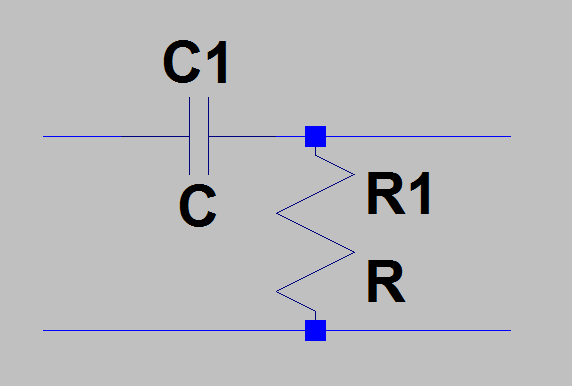
\includegraphics[width=\textwidth]{images/hochpass}
%			\end{center}
%			\caption{Hochpass}
%			\end{subfigure}
%			\begin{subfigure}{0.5\textwidth}
%			\begin{center}
%			\begin{circuitikz}
%			\draw
%			(0,0)node(gnd) {}
%			(0,2)node(C){}
%			(2,2)node(Ro){}
%			(2,0)node(Ru){}
%			(3,2)node(Uo){}
%			(3,0)node(Uu){}
%			(C) to [R=$R$, o-*] (Ro)
%			to [C=$C$,*-*] (Ru)
%			to [short, *-o] (gnd)
%			(Cu) to [short, *-o] (Uu)
%			(Co) to [short, *-o] (Uo)
%			(R) to [open, v>=$U_{\mathrm{e}}$] (gnd)
%			(Uu) to [open, v=$U_{\mathrm{a}}$] (Uo)
%			;
%			\end{circuitikz}
%			%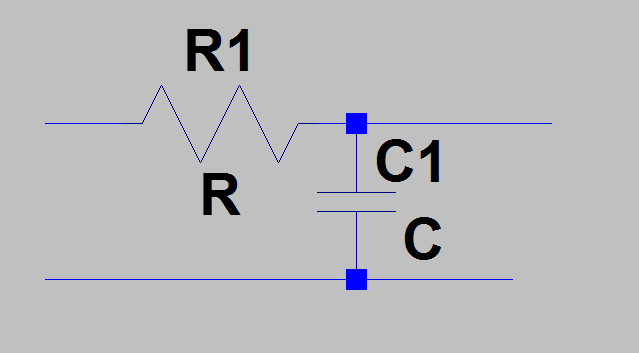
\includegraphics[width=\textwidth]{images/tiefpass}
%			\end{center}
%			\caption{Tiefpass}
%			\end{subfigure}
%		\end{figure}
		\begin{figure}[h]
		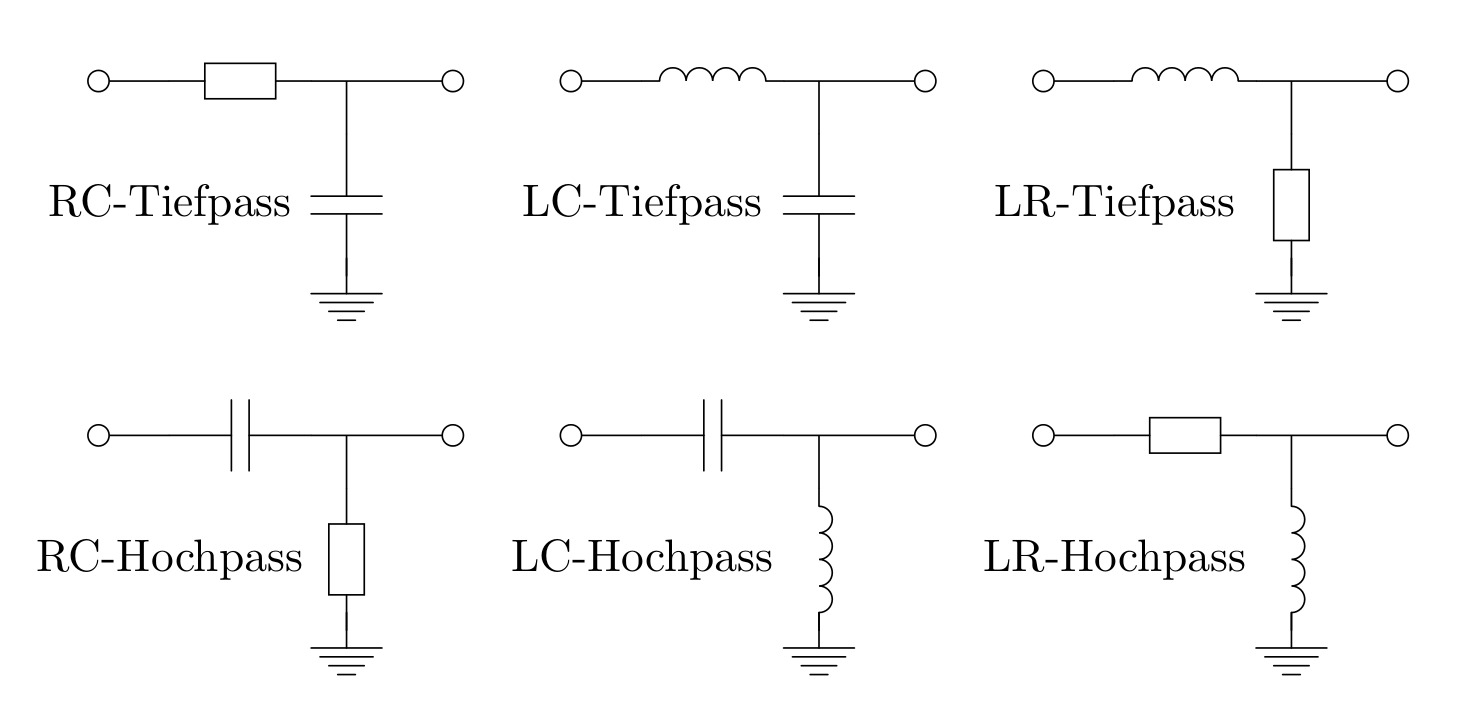
\includegraphics[width=\textwidth]{images/TP-HP-USW.png}
		\caption{Diverse Pässe}
		\end{figure}

		\subsubsection{Übertragungsfunktion}
			\begin{table}[h]
			\begin{tabular}{ll}
				Hochpass & Tiefpass\\
				\toprule
				$A_{\mathrm{HP}}=\frac{j\omega RC}{1+j\omega RC}$ & $A_{\mathrm{TP}}=\frac{1}{1+j\omega RC}$\\
				\midrule
				$\left|A\right|=\frac{\omega RC}{\sqrt{1+(\omega RC)^2}}$ & $\left|A\right|=\frac{1}{\sqrt{1+(\omega RC)^2}}$\\
				\midrule
				$\varphi=\arctan\left(\frac{1}{\omega RC}\right)$ & $\varphi=-\arctan\omega RC$\\
				\midrule
				$\omega_{\mathrm{G}}=\frac{1}{RC}$ & $\omega_{\mathrm{G}}=\frac{1}{RC}$\\
			\end{tabular}
			\end{table}
	\clearpage

	\section{Kondensator und Spule}
		\begin{table}[here]
		\begin{tabular}{lll}
		& Kondensator & Spule\\
		\toprule
		Allgemeine Formel & $(Y(0)-Y(\infty))\cdot e^{-\frac{t}{\tau}}+Y(\infty)$ & \\
		\midrule
		Ladung & $U_{\mathrm{C}}=U\left(1-e^{-\frac{t}{\tau}}\right)$ & $I_{\mathrm{L}}=\frac{U}{R}\left(1-e^{-\frac{t}{\tau}}\right)$\\
		\midrule
		Entladung & $U_{\mathrm{C}}=Ue^{-\frac{t}{\tau}}$ & $I_{\mathrm{L}}=I_0e^{-\frac{t}{\tau}}$\\
		\midrule
		Zeitkonstante & $\tau=RC$ & $\tau=\frac{R}{L}$\\
		\midrule
		Reduziert & Spannungsspitzen & Stromspitzen\\
		\end{tabular}
		\end{table}	

\section{Dioden}
	\subsection{Strom und Spannung}
		\begin{align*}
			I&=I_{R0}\cdot\left(e^{\frac{U}{mU_T}}-1\right) 
			& U&=mU_T\cdot\ln\left(\frac{I}{I_{R0}}+1\right) 
			& U\approx mU_T\cdot\ln\left(\frac{I}{I_{R0}}\right)+I\cdot R_{\mathrm{B}}
		\end{align*}

		\begin{table}[h]
		\begin{tabular}{ll}
		$U_{\mathrm{T}}\dots$ Temperaturspannung & $R_{\mathrm{B}}\dots$ Bahnwiderstand\\
		$I_{\mathrm{R}0}\dots$ Sättigungsstrom& $m\dots$ Vorfaktor (meistens 1)\\
		\end{tabular}
		\end{table}

	\subsection{Zenerdiode}
		\begin{align*}
			TK_{\mathrm{U}}&=\frac{\mathrm{d}U_{Z0}}{\mathrm{d}T}\cdot\frac{1}{U_{Z0}}
			& S^*&=S\cdot\frac{U_{\mathrm{A}}}{U_{\mathrm{E}}}
			& G&=S=\frac{\Delta U_{\mathrm{E}}}{\Delta U_{\mathrm{A}}}=1+\frac{R_{\mathrm{v}}}{r_{\mathrm{Z}}}+\frac{R_{\mathrm{v}}}{R_{\mathrm{L}}}
		\end{align*}

		\begin{table}[h]
		\begin{tabular}{ll}
		$TK_{\mathrm{U}}\dots$ Temperaturkoeffizient der Zenerspannung & $U_{Z0}\dots$ Zenerspannung\\
		$S^*\dots$ Stabilisierungsfaktor & $G=S\dots$ Glättungsfaktor\\
		\end{tabular}
		\end{table}

		\subsubsection{Widerstand}
			\begin{align*}
				R_{\mathrm{th}}&=\frac{\Delta T}{P} & r_{z\mathrm{th}}&=TK_{\mathrm{U}}\cdot U_{Z0}^2\cdot R_{\mathrm{th}}
			\end{align*}

			\begin{table}[h]
			\begin{tabular}{ll}
			$R_{\mathrm{th}}\dots$ Thermischer Widerstand & $r_{z\mathrm{th}}\dots$ Temperaturbedingter Zusatzwiderstand der Zenerdiode\\
			\end{tabular}
			\end{table}
		\clearpage

\subsection{Operationsverstärker}
	\subsection{Schaltbilder}

	\begin{figure}[h]
	\begin{subfigure}{0.25\textwidth}
		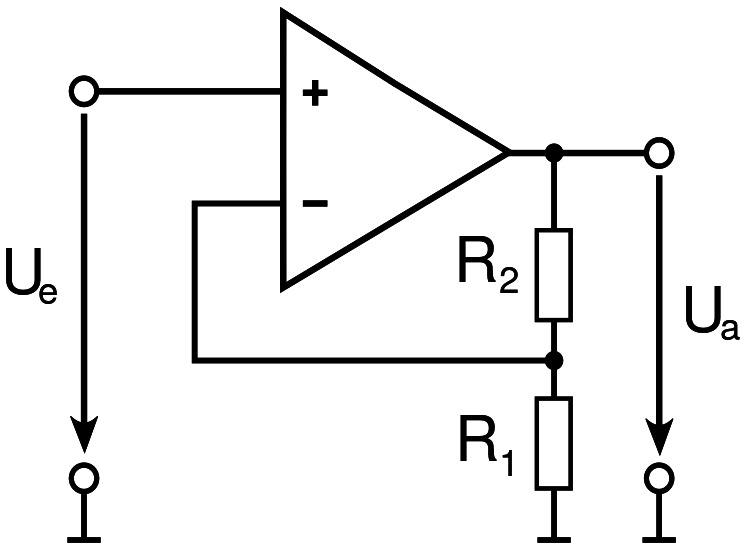
\includegraphics[width=\textwidth]{images/Noninverting_Amplifier}
		\caption{Nicht invertierender Verstärker}
	\end{subfigure}
	\begin{subfigure}{0.25\textwidth}
		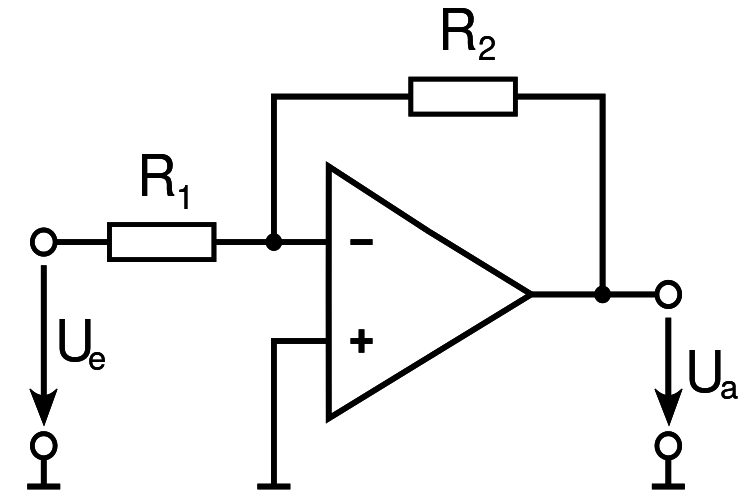
\includegraphics[width=\textwidth]{images/Inverting_Amplifier}
		\caption{Invertierender Verstärker}
	\end{subfigure}
	\begin{subfigure}{0.25\textwidth}
		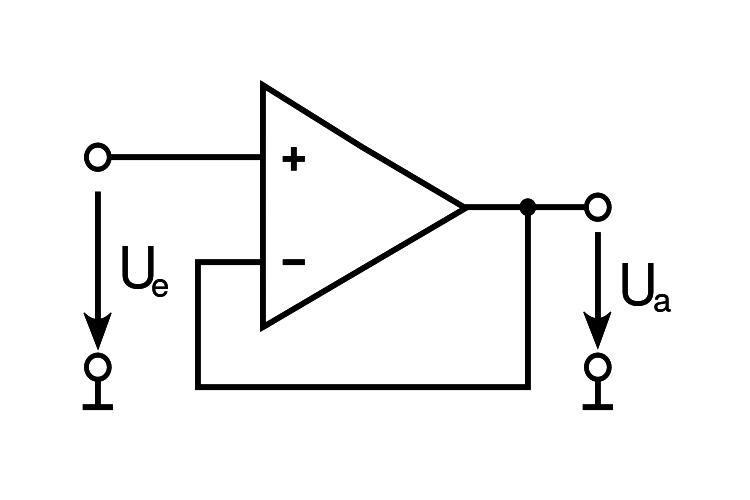
\includegraphics[width=\textwidth]{images/impedanzwandler}
		\caption{Impedanzwandler}
	\end{subfigure}
	\end{figure}
	
	\begin{figure}[h]
		\begin{subfigure}{0.25\textwidth}
		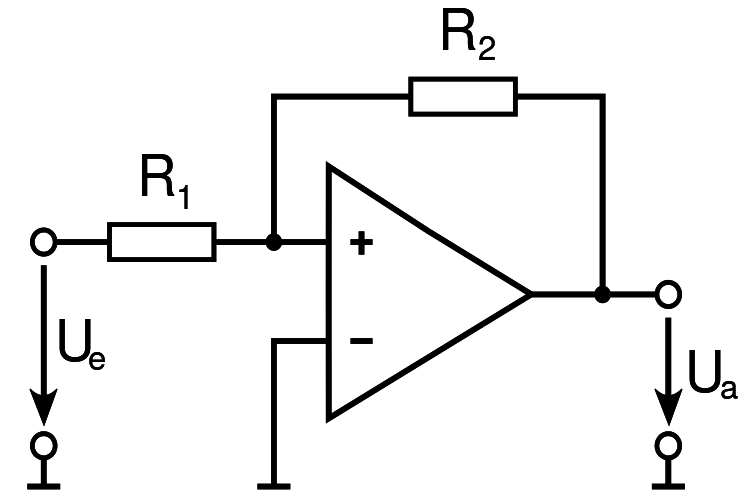
\includegraphics[width=\textwidth]{images/schmitt_noninv}
		\caption{Nicht invertierender Schmitt-Trigger}
		\end{subfigure}
		\begin{subfigure}{0.25\textwidth}
		\includegraphics[width=\textwidth]{images/schmitt_inv}
		\caption{Invertierender Schmitt-Trigger}
		\end{subfigure}
		\begin{subfigure}{0.25\textwidth}
		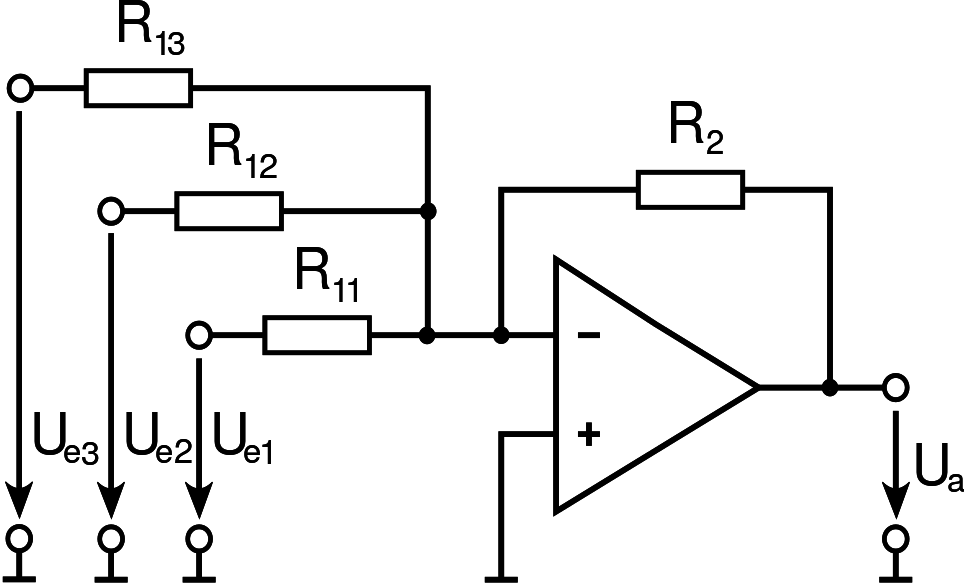
\includegraphics[width=\textwidth]{images/Inverting_Adder}
		\caption{Invertierender Addierer}
		\end{subfigure}
	\end{figure}
	\begin{figure}[h]
		\begin{subfigure}{0.25\textwidth}
		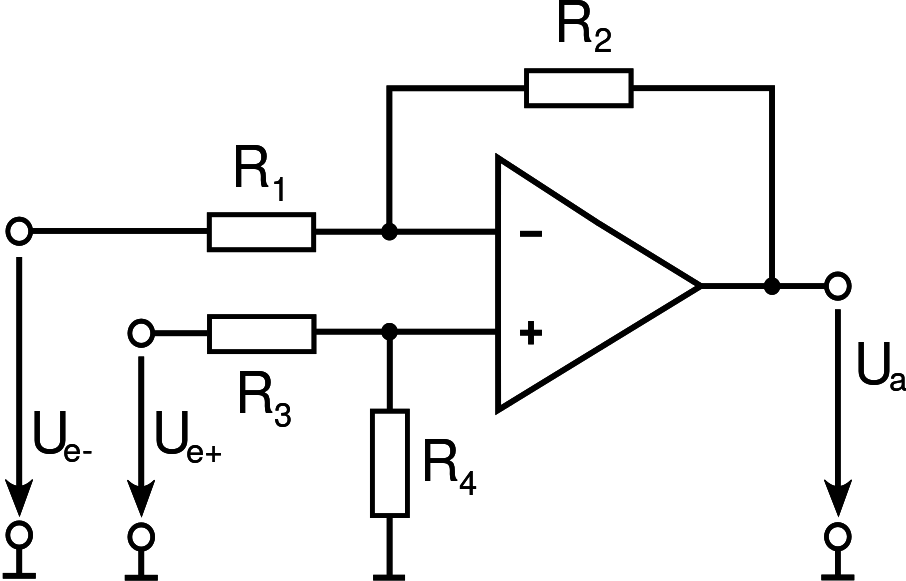
\includegraphics[width=\textwidth]{images/Differential_Amplifier}
		\caption{Subtrahierer (Differenzverstärker)}
		\end{subfigure}
		\begin{subfigure}{0.25\textwidth}
		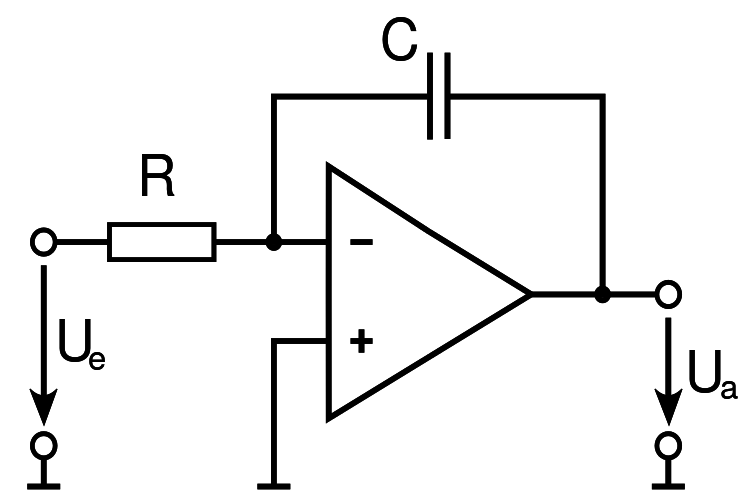
\includegraphics[width=\textwidth]{images/Integrating_Amplifier}
		\caption{Integrierer}
		\end{subfigure}
		\begin{subfigure}{0.25\textwidth}
		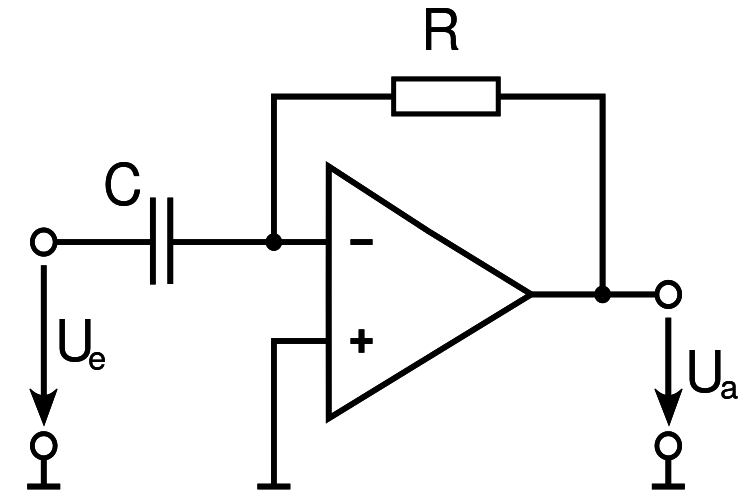
\includegraphics[width=\textwidth]{images/Differentiating_Amplifier}
		\caption{Differenzierer}
		\end{subfigure}
	\end{figure}
	\begin{figure}[h]
		\begin{subfigure}{0.25\textwidth}
		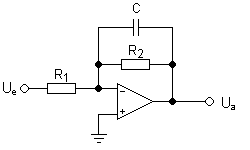
\includegraphics[width=\textwidth]{images/Aktiver_Tiefpass}
		\caption{Tiefpass}
		\end{subfigure}
		\begin{subfigure}{0.25\textwidth}
		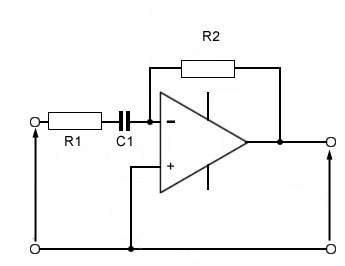
\includegraphics[width=\textwidth]{images/aktiver_hochpass}
		\caption{Hochpass}
		\end{subfigure}
		\begin{subfigure}{0.25\textwidth}
		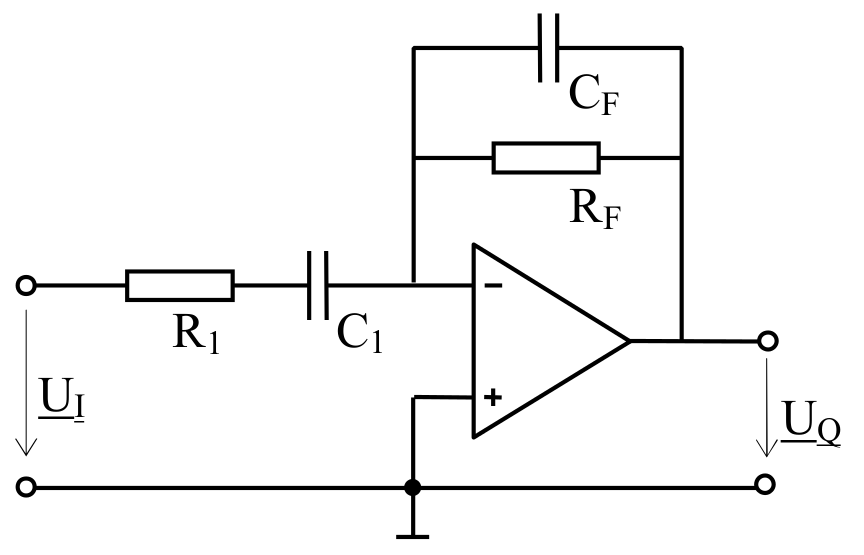
\includegraphics[width=\textwidth]{images/Bandpass}
		\caption{Bandpass}
		\end{subfigure}
	\end{figure}
\clearpage
	\begin{figure}[h]
		\begin{subfigure}{0.25\textwidth}
		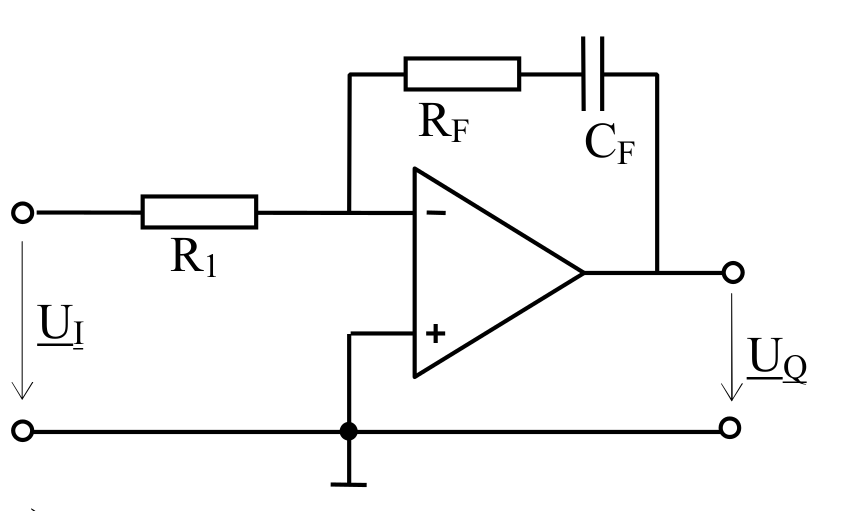
\includegraphics[width=\textwidth]{images/pi-regler}
		\caption{P-I-Regler}
		\end{subfigure}
	\end{figure}


	\subsection{Formeln}
		\begin{table}[h]
		\begin{tabularx}{\textwidth}{XXXX}
		& Nicht inv. Verst. & Inv. Verst. & Impedanzwandler\\
		\toprule
		Verstärkung & $V=\frac{u_{\mathrm{a}}}{u_{\mathrm{e}}}=1+\frac{R_2}{R_1}$ & $V=\frac{u_{\mathrm{a}}}{u_{\mathrm{e}}}=-\frac{R_2}{R_1}$ &1\\
		\midrule
		Eingangswiderstand & $\rightarrow \infty$ & $\approx R_1$ & $\rightarrow \infty$\\
		\bottomrule
		\end{tabularx}
		\end{table}
		
		\begin{table}[h]
		\begin{tabularx}{\textwidth}{XXX}
		Schaltung & Ausgangsspannung & Verstärkung / Zusätze\\
		\toprule
		Schmitt-Trigger (inv.) & $U_{\mathrm{S}1,2}=\frac{U_{\mathrm{QM}\pm}\cdot R_1+U_{\mathrm{Ref}}\cdot R_2}{R_1+R_2}$
		& $\Delta U_{\mathrm{Hyst}}=\frac{2U_{\mathrm{a}}R_1}{R_1+R_2}$\\
		\midrule
		Inv. Verst. & $U_{\mathrm{a}}=-U_{\mathrm{e}}\frac{R_2}{R_1}$ 
		& $V_{\mathrm{U}}=\frac{U_{\mathrm{a}}}{U_{\mathrm{e}}}=-\frac{R_2}{R_1}$\\
		\midrule
		Nicht inv. Verst. & $U_{\mathrm{a}}=U_{\mathrm{e}}\cdot\left(1+\frac{R_2}{R_1}\right)$ 
		& $V_{\mathrm{U}}=\frac{U_{\mathrm{a}}}{U_{\mathrm{e}}}=1+\frac{R_2}{R_1}$\\
		\midrule
		Addierer & $U_{\mathrm{a}}=-\left(\sum_{i=1}^3 U_{\mathrm{e}i}\cdot\frac{R_2}{R_{1i}}\right)$ 
		& $V_{\mathrm{U}}=-\frac{R_2}{R1} \Leftrightarrow R_i=R_1$\\
		\midrule
		Subtrahierer & $U_{\mathrm{a}}=$ & \\
		& $\left(U_{\mathrm{e}+}\cdot\frac{R_1+R_2}{R_3+R_4}\cdot\frac{R_4}{R_1}-U_{\mathrm{e}-}\cdot\frac{R_2}{R_1}\right)$ &\\
		\midrule
		Integrierer & $u_{\mathrm{a}}=-\frac{1}{RC}\int u_{\mathrm{e}} \mathrm{d}t$ 
		& $|V_{\mathrm{U}}|=\frac{\hat{u}_{\mathrm{a}}}{\hat{u}_{\mathrm{e}}}=\frac{1}{\omega RC}=f(\omega)$\\
		\midrule
		Differenzierer & $u_{\mathrm{a}}=-RC\cdot\frac{\mathrm{d}u_{\mathrm{e}}}{\mathrm{d}t}$ &
		$|V_{\mathrm{U}}|=\frac{\hat{u}_{\mathrm{a}}}{\hat{u}_{\mathrm{e}}}\approx\omega RC=f(\omega)$\\
		\midrule
		Tiefpass & $\underline{U}_{\mathrm{a}}=-\underline{U}_{\mathrm{e}}\frac{\underline{Z}_2}{\underline{Z}_1}$ 
		& $\left|\frac{V_{\mathrm{U}}(\omega)}{V_{\mathrm{U}}(0)}\right|=\frac{1}{\sqrt{1+\Omega^2}}$\\
		& & $\Omega=\frac{\omega}{\omega_{\mathrm{G}}} \& \omega_{\mathrm{G}}=\frac{1}{R_2C}$\\
		\midrule
		Hochpass & $\underline{U}_{\mathrm{a}}=-\underline{U}_{\mathrm{e}}\frac{\underline{Z}_2}{\underline{Z}_1}$ 
		& $\underline{U}_{\mathrm{a}}=-\underline{U}_{\mathrm{e}}\frac{R_2}{R_1}\frac{1}{1-j\left(\frac{1}{\Omega}\right)}$ \\
		& & $\Omega=\frac{\omega}{\omega_{\mathrm{G}}}\&\omega_{\mathrm{G}}=\frac{1}{R_1C}$ \\
		\midrule
		PI-Regler & $\underline{U}_{\mathrm{a}}=\underline{U}_{\mathrm{e}}\left(-\frac{R_2}{R_1}+j\frac{1}{\omega C R_1}\right)$ &\\
		\bottomrule
		\end{tabularx}
		\end{table}

		\begin{table}[h]
		\begin{tabular}{lll}
		$U_{\mathrm{e}}\dots$ Eingangsspannung & $U_{\mathrm{a}}\dots$ Ausgangsspannung & $U_{\mathrm{S}}\dots$ Schaltschwelle\\
		$\Delta U_{\mathrm{Hyst}}\dots$ Hysterese & $\omega_{\mathrm{G}}\dots$ Grenzkreisfrequenz & $\Omega\dots$ Normierte Frequenz\\
		\end{tabular}
		\end{table}
\clearpage

\section{Bipolartransistoren}
	\subsection{Schaltungen}
		\begin{figure}[h]
			\begin{subfigure}{0.3\textwidth}
			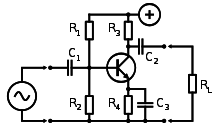
\includegraphics[width=\textwidth]{images/emitterschaltung}
			\begin{center}
			\caption{Emitterschaltung mit Arbeitspunkteinstellung}
			\end{center}
			\end{subfigure}
			\begin{subfigure}{0.3\textwidth}
			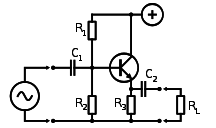
\includegraphics[width=\textwidth]{images/kollektorschaltung}
			\begin{center}
			\caption{Kollektorschaltung}
			\end{center}
			\end{subfigure}
			\begin{subfigure}{0.3\textwidth}
			\begin{center}
			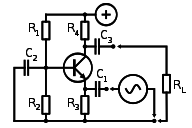
\includegraphics[width=\textwidth]{images/basisschaltung}
			\caption{Basisschaltung}
			\end{center}
			\end{subfigure}
		\end{figure}
		
		\begin{figure}[h]
			\begin{subfigure}{0.5\textwidth}
			%\input{images/kleinsignal}
			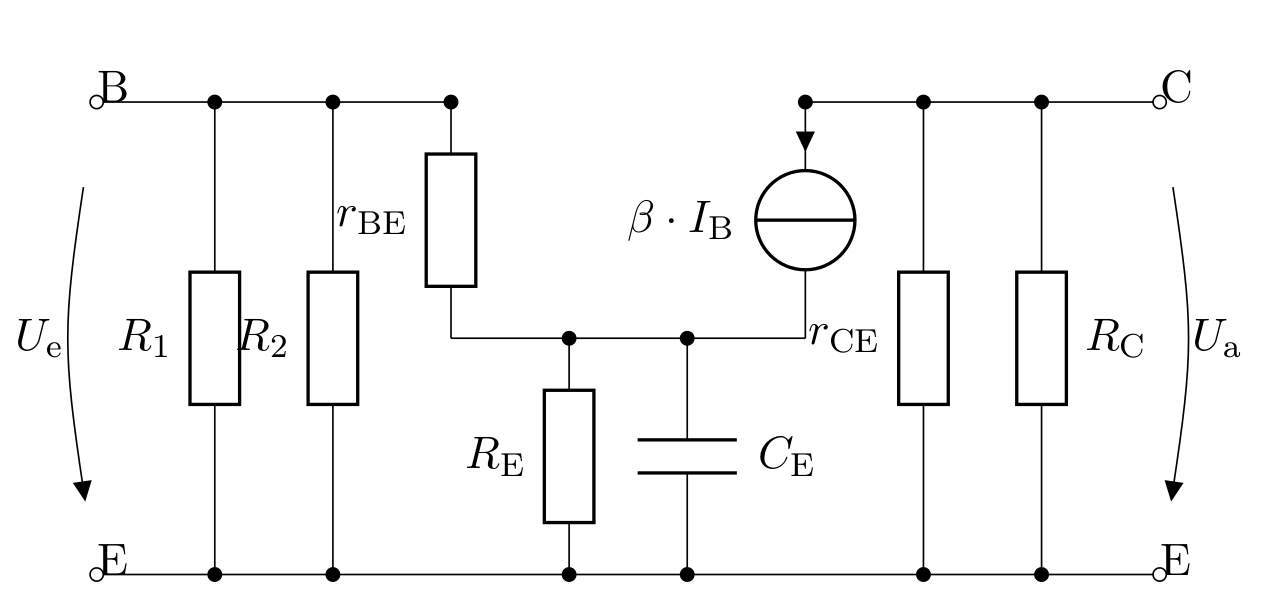
\includegraphics[width=\textwidth]{images/kleinsignal}
			\caption{Kleinsignalersatzschaltbild}
			\end{subfigure}
			\begin{subfigure}{0.5\textwidth}
			%\input{images/gl}
			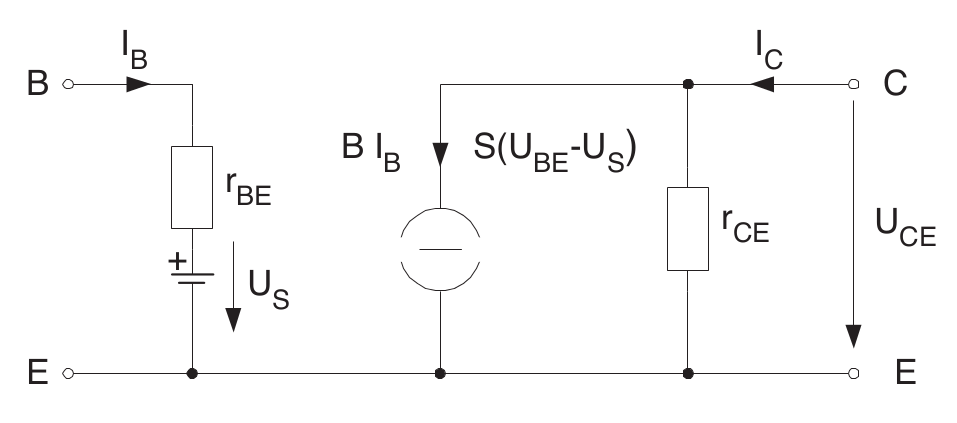
\includegraphics[width=\textwidth]{images/gleichstrom}
			\caption{Gleichstromersatzschaltbild}
			\end{subfigure}
		\end{figure}

	\subsection{Formeln}
		\subsubsection{Ströme}
			\begin{align*}
				I_{\mathrm{C}}&=B\cdot I_{\mathrm{B}} 
				& I_{\mathrm{B}}&=I_{\mathrm{S}}\cdot\left(e^{\frac{U_{\mathrm{BE}}}{U_{\mathrm{T}}}}-1\right) 
				& I_{\mathrm{E}}=I_{\mathrm{C}}+I_{\mathrm{B}} 
			\end{align*}
			\begin{table}[h]
			\begin{tabular}{ll}
			$I_{\mathrm{C}}\dots$ Kollektorstrom & $U_{\mathrm{T}}\dots$ Temperaturspannung, $86\mu\mathrm{V}\cdot\nicefrac{T}{\mathrm{K}}$, 26mV bei Raumtemperatur (300K)\\
			$I_{\mathrm{B}}\dots$ Basisstrom & $U_{\mathrm{BE}}\dots$ Basis-Emitterspannung, siehe Schaltbild
\\
			$I_{\mathrm{E}}\dots$ Emitterstrom & \\
			\end{tabular}
			\end{table}

		\subsubsection{Widerstände}
			\begin{align*}
				r_{\mathrm{BE}}\approx\frac{\Delta U_{\mathrm{BE}}}{\Delta I_{\mathrm{B}}}=\frac{U_{\mathrm{T}}}{I_{\mathrm{B}}} 
				&& r_{\mathrm{CE}}&=\frac{\Delta U_{\mathrm{CE}}}{\Delta I_{\mathrm{C}}}
			\end{align*}
			\begin{table}[h]
			\begin{tabular}{ll}
			$r_{\mathrm{BE}}\dots$ Basis-Emitter-Widerstand & $r_{\mathrm{CE}}\dots$ Kollektor-Emitter-Widerstand\\
			\end{tabular}
			\end{table}

		\subsubsection{Verstärkungen}
			\begin{align*}
				S&=\frac{\mathrm{d}I_{\mathrm{C}}}{\mathrm{d}U_{\mathrm{BE}}}\approx\frac{\Delta I_{\mathrm{C}}}{\Delta U_{\mathrm{BE}}}=\frac{I_{\mathrm{C}}}{U_{\mathrm{T}}} 
				& \beta\approx\frac{\Delta I_{\mathrm{C}}}{\Delta I_{\mathrm{B}}}
			\end{align*}
		
		\subsubsection{Early-Effekt}
			\begin{align*}
				I_{\mathrm{C}}&=B\cdot I_{\mathrm{B}}\cdot(1+\lambda U_{\mathrm{CE}})=B\cdot I_{\mathrm{B}}+\frac{U_{\mathrm{CE}}}{r_{\mathrm{CE}}} 
				& r_{\mathrm{CE}}&=\frac{\Delta U_{\mathrm{CE}}}{\Delta I_{\mathrm{C}}}=\frac{U_{\mathrm{y}}+U_{\mathrm{CE}}}{I_{\mathrm{C}}}=\frac{U_{\mathrm{y}}}{B\cdot I_{\mathrm{B}}}
				& \frac{1}{\lambda} &= U_{\mathrm{y}}
			\end{align*}

			$U_{\mathrm{y}}\dots$ Early-Spannung, ihr Fehlen weist auf Vernachlässigung des Early-Effekts hin $\Leftrightarrow$ kein $r_{\mathrm{CE}} \Leftrightarrow$ Transistor idealer Leiter

		\subsubsection{Emitterschaltung}
			\begin{align*}
				U_{\mathrm{B}}&=U_{\mathrm{CE}}+I_{\mathrm{C}}\cdot R_{\mathrm{C}} 
				& U_{\mathrm{a}}&=U_{\mathrm{CE}} & \Delta U_{\mathrm{a}}&=-\Delta I_{\mathrm{C}}\cdot R_{\mathrm{C}} 
				& S=\frac{\Delta I_{\mathrm{C}}}{\Delta U_{\mathrm{BE}}}\\
				\Delta U_{\mathrm{a}}&=-\Delta U_{\mathrm{e}}\cdot S\cdot R_{\mathrm{C}} 
				& v_{\mathrm{u}}&=\frac{\Delta U_{\mathrm{a}}}{\Delta U_{\mathrm{e}}}=-S\cdot R_{\mathrm{C}}
			\end{align*}
			\begin{table}[h]
			\begin{tabular}{ll}
			$S\dots$ Steilheit & $v_{\mathrm{u}}\dots$ Spannungsverstärkung\\
			$U_{\mathrm{a}}\dots$ Ausgangsspannung & $U_{\mathrm{e}}\dots$ Eingangsspannung\\
			\end{tabular}
			\end{table}

\input{content/chapters/fet}


% Hier kommmen Tabellen und Bilder
%\listoftables
%\listoffigures

\end{document}
%% Dokument ENDE %%%%%%%%%%%%%%%%%%%%%%%%%%%%%%%%%%%%%%%%%%%%%%%%%%%%%%%%%%

